\documentclass[border=4pt]{standalone}
\usepackage{amsmath,amssymb,amsfonts}
\usepackage{xcolor,colortbl,array,booktabs,multirow}
\usepackage{tikz}
\usetikzlibrary{arrows, automata, backgrounds, calendar, chains, decorations,
    matrix, mindmap, patterns, petri, positioning, shadows, shapes.geometric,
    trees, shapes, decorations.pathreplacing, calc, tikzmark, arrows.meta}
\newcommand{\st}{\text{ s.t. }}
\newcommand{\x}{\mathbf{x}}
\renewcommand{\b}{\mathbf{b}}
\newcommand{\A}{\mathbf{A}}
\newcommand{\R}{\mathbb{R}}
\newcommand{\RR}{\mathbb{R}}
\newcommand{\Z}{\mathbb{Z}}
\newcommand{\ZZ}{\mathbb{Z}}
\begin{document}
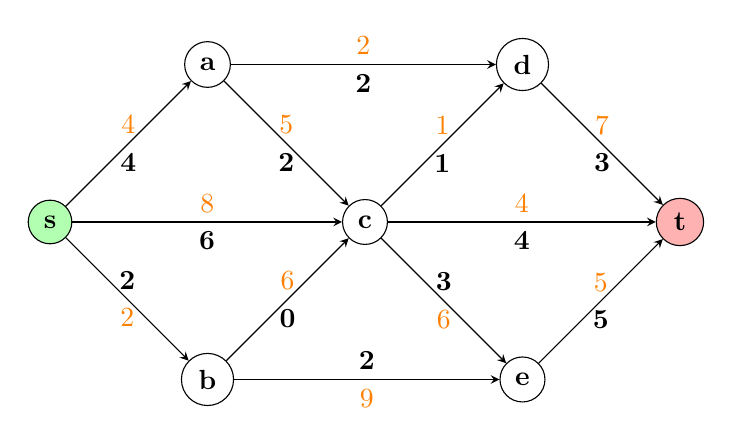
\begin{tikzpicture}[>=stealth, node distance=2cm]

    % Nodes with specific styles
    \node[draw, circle, fill=green,
         fill opacity = 0.3,  text opacity=1] (s) at (0,2) {\textbf{s}};
    \node[draw, circle] (a) at (2,4) {\textbf{a}};
    \node[draw, circle] (b) at (2,0) {\textbf{b}};
    \node[draw, circle] (c) at (4,2) {\textbf{c}};
    \node[draw, circle] (d) at (6,4) {\textbf{d}};
    \node[draw, circle] (e) at (6,0) {\textbf{e}};
    \node[ fill=red,
         fill opacity = 0.3, draw, circle,  text opacity=1] (t) at (8,2) {\textbf{t}};

    % Edges with costs (orange, upright) and flows (bold black, below)
    \draw[->] (s) -- (a) node[midway, above, text=orange] {4} 
                         node[midway, below, text=black] {\textbf{4}};
    \draw[->] (s) -- (c) node[midway, above, text=orange] {8} 
                         node[midway, below, text=black] {\textbf{6}};
    \draw[->] (s) -- (b) node[midway, below, text=orange] {2} 
                         node[midway, above, text=black] {\textbf{2}};
    
    \draw[->] (a) -- (c) node[midway, above, text=orange] {5} 
                         node[midway, below, text=black] {\textbf{2}};
    \draw[->] (a) -- (d) node[midway, above, text=orange] {2} 
                         node[midway, below, text=black] {\textbf{2}};

    \draw[->] (c) -- (d) node[midway, above, text=orange] {1} 
                         node[midway, below, text=black] {\textbf{1}}; % Adjusted to respect capacity
    \draw[->] (c) -- (t) node[midway, above, text=orange] {4} 
                         node[midway, below, text=black] {\textbf{4}};
    \draw[->] (c) -- (e) node[midway, below, text=orange] {6} 
                         node[midway, above, text=black] {\textbf{3}};

    \draw[->] (b) -- (c) node[midway, above, text=orange] {6} 
                         node[midway, below, text=black] {\textbf{0}};
    \draw[->] (b) -- (e) node[midway, below, text=orange] {9} 
                         node[midway, above, text=black] {\textbf{2}};

    \draw[->] (d) -- (t) node[midway, above, text=orange] {7} 
                         node[midway, below, text=black] {\textbf{3}};
    \draw[->] (e) -- (t) node[midway, above, text=orange] {5} 
                         node[midway, below, text=black] {\textbf{5}};

\end{tikzpicture}
\end{document}
